\documentclass[11pt,handout]{beamer}

\usepackage{tcolorbox}
\usepackage{minted}
\usepackage{pdfpages}
\usepackage{sourcecodepro}
\usepackage{graphicx}
\usepackage{amsmath}
\usepackage{fullpage}
\usepackage{bussproofs}
\usepackage{mathpartir}
\usepackage{prooftrees}
\usepackage{color}
\usepackage{algorithmicx}
\usepackage{algpseudocode}

\usetikzlibrary{calc}

\graphicspath{{img/}}

\usetheme{CambridgeUS}
\setbeamertemplate{\insertframenumber/\inserttotalframenumber}

\title[Computer Chess]{Bisimulation Minimization and Symbolic Model Checking}
\author{Sylvain Julmy}
\date{\today}

\begin{document}

\maketitle

\begin{frame}[fragile]
  \frametitle{Bisimulation minimization}
  \begin{figure}[h]
  \centering
  \fbox{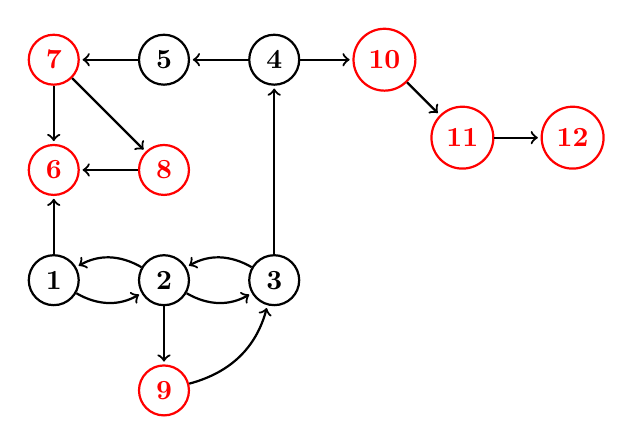
\begin{tikzpicture}[->,shorten >=1pt,auto,node distance=1.4cm,
                thick,main node/.style={circle,draw,font=\bfseries}]
	\node[main node,red] (1) {7};
	\node[main node,red] (2) [below of = 1] {6};
	\node[main node] (3) [below of = 2] {1};
	\node[main node] (4) [right of = 1] {5};
	\node[main node,red] (5) [below of = 4] {8};
	\node[main node] (6) [below of = 5] {2};
	\node[main node,red] (7) [below of = 6] {9};
	\node[main node] (8) [right of = 4] {4};
	\node[main node,red] (9) [right of = 8] {10};
	\node[main node,red] (10) [below right of = 9] {11};
	\node[main node] (11) [right of = 6] {3};
	\node[main node,red] (12) [right of = 10] {12};
	
	\path
	(1) edge node {} (2)
	(1) edge node {} (5)
	(5) edge node {} (2)
	(3) edge node {} (2)
	(6) edge [bend right] node {} (3)
	(3) edge [bend right] node {} (6)
	(6) edge node {} (7)
	(7) edge [bend right] node {} (11)
	(11) edge [bend right] node {} (6)	
	(6) edge [bend right] node {} (11)
	(11) edge node {} (8)
	(8) edge node {} (4)
	(4) edge node {} (1)
	(8) edge node {} (9)
	(9) edge node {} (10)
	(10) edge node {} (12)
;
\end{tikzpicture}}
  \caption{Initial state}
  \label{fig:bisimulation_minimization_1}
\end{figure}
\end{frame}

\begin{frame}[fragile]
  \frametitle{Bisimulation minimization}
  \begin{figure}[h]
  \centering
  \fbox{\usetikzlibrary{calc}
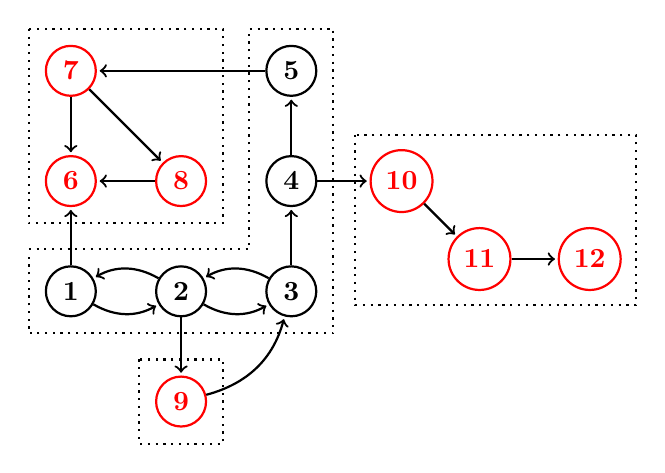
\begin{tikzpicture}[shorten >=1pt,auto,node distance=1.4cm,
                thick,main node/.style={circle,draw,font=\bfseries}]
	\node[main node,red] (1) {7};
	\node[main node,red] (2) [below of = 1] {6};
	\node[main node] (3) [below of = 2] {1};
	\node[main node,red] (5) [right of = 2] {8};
	\node[main node] (6) [below of = 5] {2};
	\node[main node,red] (7) [below of = 6] {9};
	\node[main node] (8) [right of = 5] {4};
	\node[main node] (4) [above of = 8] {5};
	\node[main node,red] (9) [right of = 8] {10};
	\node[main node,red] (10) [below right of = 9] {11};
	\node[main node] (11) [right of = 6] {3};
	\node[main node,red] (12) [right of = 10] {12};
	
	\path[->]
	(1) edge node {} (2)
	(1) edge node {} (5)
	(5) edge node {} (2)
	(3) edge node {} (2)
	(6) edge [bend right] node {} (3)
	(3) edge [bend right] node {} (6)
	(6) edge node {} (7)
	(7) edge [bend right] node {} (11)
	(11) edge [bend right] node {} (6)	
	(6) edge [bend right] node {} (11)
	(11) edge node {} (8)
	(8) edge node {} (4)
	(4) edge node {} (1)
	(8) edge node {} (9)
	(9) edge node {} (10)
	(10) edge node {} (12);
	
	\draw[black,thick,dotted] ($(1.north west)+(-0.3,0.3)$)  rectangle ($(5.south east)+(0.3,-0.3)$);
	\draw[black,thick,dotted] ($(3.north west)+(-0.3,0.3)$)  -- 
											  ($(11.north west)+(-0.3,0.3)$) --
											  ($(4.north west)+(-0.3,0.3)$) --
											  ($(4.north east)+(+0.3,0.3)$) --
											  ($(11.south east) + (0.3,-0.3)$) --
			 								  ($(3.south west)+(-0.3,-0.3)$) --
											  ($(3.north west)+(-0.3,0.3)$);
	\draw[black,thick,dotted] ($(7.north west)+(-0.3,0.3)$)  rectangle ($(7.south east)+(0.3,-0.3)$);
	\draw[black,thick,dotted] ($(9.north west)+(-0.3,0.3)$)  rectangle ($(12.south east)+(0.3,-0.3)$);

\end{tikzpicture}}
  \caption{Initial partition block}
  \label{fig:bisimulation_minimization_2}
\end{figure}
\end{frame}

\begin{frame}[fragile]
  \frametitle{Bisimulation minimization}
  \begin{figure}[h]
  \centering
  \fbox{\usetikzlibrary{calc}
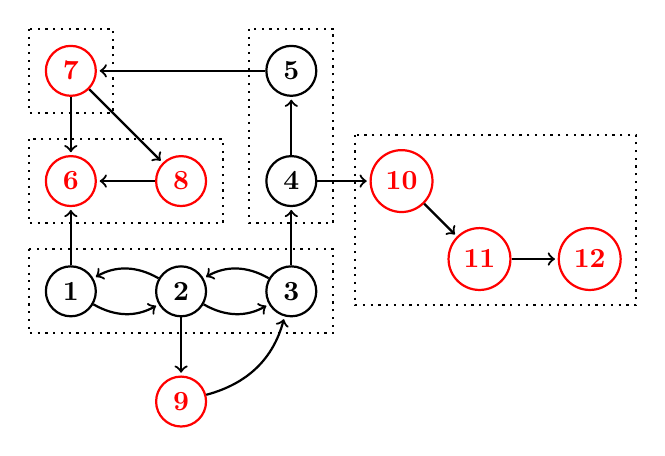
\begin{tikzpicture}[shorten >=1pt,auto,node distance=1.4cm,
                thick,main node/.style={circle,draw,font=\bfseries}]
	\node[main node,red] (1) {7};
	\node[main node,red] (2) [below of = 1] {6};
	\node[main node] (3) [below of = 2] {1};
	\node[main node,red] (5) [right of = 2] {8};
	\node[main node] (6) [below of = 5] {2};
	\node[main node,red] (7) [below of = 6] {9};
	\node[main node] (8) [right of = 5] {4};
	\node[main node] (4) [above of = 8] {5};
	\node[main node,red] (9) [right of = 8] {10};
	\node[main node,red] (10) [below right of = 9] {11};
	\node[main node] (11) [right of = 6] {3};
	\node[main node,red] (12) [right of = 10] {12};
	
	\path[->]
	(1) edge node {} (2)
	(1) edge node {} (5)
	(5) edge node {} (2)
	(3) edge node {} (2)
	(6) edge [bend right] node {} (3)
	(3) edge [bend right] node {} (6)
	(6) edge node {} (7)
	(7) edge [bend right] node {} (11)
	(11) edge [bend right] node {} (6)	
	(6) edge [bend right] node {} (11)
	(11) edge node {} (8)
	(8) edge node {} (4)
	(4) edge node {} (1)
	(8) edge node {} (9)
	(9) edge node {} (10)
	(10) edge node {} (12);

	\draw[black,thick,dotted] ($(1.north west)+(-0.3,0.3)$)  rectangle ($(1.south east)+(0.3,-0.3)$);
	\draw[black,thick,dotted] ($(2.north west)+(-0.3,0.3)$)  rectangle ($(5.south east)+(0.3,-0.3)$);
	\draw[black,thick,dotted] ($(3.north west)+(-0.3,0.3)$)  rectangle ($(11.south east)+(0.3,-0.3)$);
	\draw[black,thick,dotted] ($(4.north west)+(-0.3,0.3)$)  rectangle ($(8.south east)+(0.3,-0.3)$);
	\draw[black,thick,dotted] ($(9.north west)+(-0.3,0.3)$)  rectangle ($(12.south east)+(0.3,-0.3)$);

\end{tikzpicture}}
  \caption{Computation of equivalence classes}
  \label{fig:bisimulation_minimization_3}
\end{figure}
\end{frame}

\begin{frame}[fragile]
  \frametitle{Bisimulation minimization}
  \begin{figure}[h]
  \centering
  \fbox{\usetikzlibrary{calc}
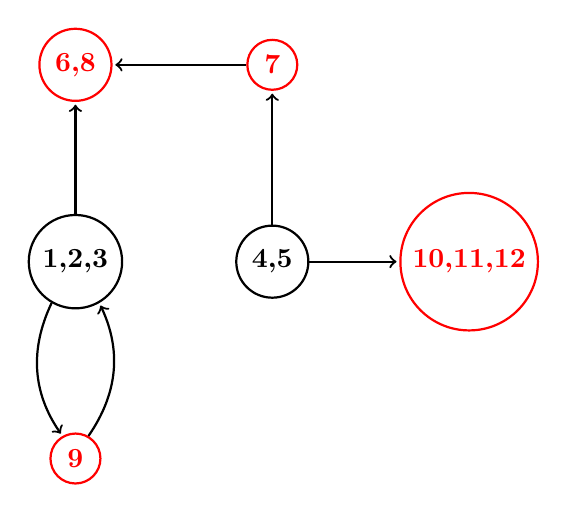
\begin{tikzpicture}[shorten >=1pt,auto,node distance=2.5cm,
                thick,main node/.style={circle,draw,font=\bfseries}]

	\node[main node,red] (1) {7};	
	\node[main node,red] (2) [left of = 1] {6,8};	
	\node[main node] (3) [below of = 2] {1,2,3};	
	\node[main node] (4) [right of = 3] {4,5};
	\node[main node,red] [below of = 3] (5) {9};
	\node[main node,red] [right of = 4] (6) {10,11,12};

	\path[->]
	(3) edge [bend right] node {} (5)
	(5) edge [bend right] node {} (3)
	(3) edge node {} (2)
	(1) edge node {} (2)
	(4) edge node {} (1)
	(4) edge node {} (6)
	;
\end{tikzpicture}}
  \caption{Final system to model check}
  \label{fig:bisimulation_minimization_4}
\end{figure}
\end{frame}

\begin{frame}
  \frametitle{BFH}
  BFH, like LY, selects reachable blocks to stabilize but differ in how to
  stabilize a block.

  \pause
  \vspace*{0.5cm}
  
  BFH stabilize a block w.r.t. all the other blocks (either reachable or
  unreachable).
  
  \pause
  \vspace*{0.5cm}
  
  The algorithm become simplier but unnecessary work is done.
\end{frame}

\begin{frame}[fragile]
  \frametitle{BFH - Algorithm}
  \begin{algorithmic}[1]
    \State $S := \emptyset$ List of stable block
    \State $R := \{[init]_p\}$ List of reachable block
    \While{$R \neq S$}
    \State Select a reachable, but unstable block $X$
    \State Stabilize $X$ w.r.t. every block in the partition
    \If{No new blocks are created}
    \State Add $X$ to $S$
    \State Block reachable from $X$ are added to $R$
    \Else
    \State Add new the new blocks to the partition
    \State Update the initial block
    \State Remove from $S$ the blocks that becomes unstable
    \EndIf
    \EndWhile
  \end{algorithmic}
\end{frame}

\begin{frame}[fragile]
  \frametitle{BFH - New Algorithm}
  \begin{algorithmic}[1]
    \State $I := [init]_p$
    \State Mark the bad block
    \While{$I$ is not marked}
    \State Stabilize $I$
    \If{No new blocks are created}
    \If{$post_p(I) \setminus \{I\} = \emptyset$}
    \State Signal safety violation
    \Else
    \State Break
    \EndIf
    \Else
    
    \EndIf
    \EndWhile
    \If{$I$ is marked}
    \State Signal safety violation
    \EndIf
  \end{algorithmic}
\end{frame}

\begin{frame}
  \frametitle{BFH - Termination}
  As in LY, BFH could terminate when a second block becomes reachable.
  
  \pause
  \vspace*{0.5cm}

  Correctly determine violations of invariants but not as soon as they occur.
\end{frame}

\begin{frame}
  \frametitle{BFH - Termination}

  The algorthim may traverse a path from the bad block to the initial state
  before the initial block becomes stable.

  \pause
  \vspace*{0.5cm}

  Thus, the algorithm take more iteration to terminate.
\end{frame}

\end{document}